%% 
%% Copyright 2007-2020 Elsevier Ltd
%% 
%% This file is part of the 'Elsarticle Bundle'.
%% ---------------------------------------------
%% 
%% It may be distributed under the conditions of the LaTeX Project Public
%% License, either version 1.2 of this license or (at your option) any
%% later version.  The latest version of this license is in
%%    http://www.latex-project.org/lppl.txt
%% and version 1.2 or later is part of all distributions of LaTeX
%% version 1999/12/01 or later.
%% 
%% The list of all files belonging to the 'Elsarticle Bundle' is
%% given in the file `manifest.txt'.
%% 

%% Template article for Elsevier's document class `elsarticle'
%% with numbered style bibliographic references
%% SP 2008/03/01
%%
%% 
%%
%% $Id: elsarticle-template-num.tex 190 2020-11-23 11:12:32Z rishi $
%%
%%
\documentclass[preprint,12pt]{elsarticle}

%% Use the option review to obtain double line spacing
%% \documentclass[authoryear,preprint,review,12pt]{elsarticle}

%% Use the options 1p,twocolumn; 3p; 3p,twocolumn; 5p; or 5p,twocolumn
%% for a journal layout:
%% \documentclass[final,1p,times]{elsarticle}
%% \documentclass[final,1p,times,twocolumn]{elsarticle}
%% \documentclass[final,3p,times]{elsarticle}
%% \documentclass[final,3p,times,twocolumn]{elsarticle}
%% \documentclass[final,5p,times]{elsarticle}
%% \documentclass[final,5p,times,twocolumn]{elsarticle}

%% For including figures, graphicx.sty has been loaded in
%% elsarticle.cls. If you prefer to use the old commands
%% please give \usepackage{epsfig}

%% The amssymb package provides various useful mathematical symbols
\usepackage{amssymb}
\usepackage{amsmath}
%% The amsthm package provides extended theorem environments
%% \usepackage{amsthm}

%% The lineno packages adds line numbers. Start line numbering with
%% \begin{linenumbers}, end it with \end{linenumbers}. Or switch it on
%% for the whole article with \linenumbers.
%% \usepackage{lineno}

\journal{LCCV}

\begin{document}

\begin{frontmatter}

%% Title, authors and addresses

%% use the tnoteref command within \title for footnotes;
%% use the tnotetext command for theassociated footnote;
%% use the fnref command within \author or \address for footnotes;
%% use the fntext command for theassociated footnote;
%% use the corref command within \author for corresponding author footnotes;
%% use the cortext command for theassociated footnote;
%% use the ead command for the email address,
%% and the form \ead[url] for the home page:
%% \title{Title\tnoteref{label1}}
%% \tnotetext[label1]{}
%% \author{Name\corref{cor1}\fnref{label2}}
%% \ead{email address}
%% \ead[url]{home page}
%% \fntext[label2]{}
%% \cortext[cor1]{}
%% \affiliation{organization={},
%%             addressline={},
%%             city={},
%%             postcode={},
%%             state={},
%%             country={}}
%% \fntext[label3]{}

\title{Unidimensional Axial Vibration Using MPM}

%% use optional labels to link authors explicitly to addresses:
%% \author[label1,label2]{}
%% \affiliation[label1]{organization={},
%%             addressline={},
%%             city={},
%%             postcode={},
%%             state={},
%%             country={}}
%%
%% \affiliation[label2]{organization={},
%%             addressline={},
%%             city={},
%%             postcode={},
%%             state={},
%%             country={}}

\author[inst1]{Adriano da Silva Rocha}

\affiliation[inst1]{organization={Laboratory of Scientific Computation and Visualization},%Department and Organization
            addressline={Av. Lourival Melo Mota, S/N}, 
            city={Maceió},
            postcode={57072-900}, 
            state={Alagoas},
            country={Brazil}}

\begin{abstract}
%% Text of abstract
The material point method (MPM) is a numerical simulation method that combines features of classical numerical methods to achieve greater applicability and efficiency. This work aimed to apply the MPM for didactic purposes to a one-dimensional system composed of a continuous bar under free axial vibration. For this, initial conditions capable of excite isolated vibration modes were considered, and for the MPM simulation, the USF (update stress first) algorithm was used. After numerical simulation for three vibration modes (1st, 5th, 10th) the center of mass velocity values were compared with analytical results. The results of the first mode of vibration were the same as the analytical solution, while the curves for the following modes showed similar amplitudes, but also an increasing phase difference according to the order of oscillation, being 5\% for the fifth mode and 20\% to the tenth mode, as found in the literature. Complementary simulations with adjustment in the spatial discretization reduced the phase difference to about 1\% for the fifth mode and 5\% for the tenth. Thus, it is observed that the application of the method was satisfactory and that its precision is dependent on the parameters used for simulation.
\end{abstract}

%%Graphical abstract
%\begin{graphicalabstract}
%\includegraphics{grabs}
%\end{graphicalabstract}

%%Research highlights
%\begin{highlights}
%\item Research highlight 1
%\item Research highlight 2
%\end{highlights}

\begin{keyword}
%% keywords here, in the form: keyword \sep keyword
Material Point Method \sep Axial Vibration \sep USF
%% PACS codes here, in the form: \PACS code \sep code
%\PACS 0000 \sep 1111
%% MSC codes here, in the form: \MSC code \sep code
%% or \MSC[2008] code \sep code (2000 is the default)
%\MSC 0000 \sep 1111
\end{keyword}

\end{frontmatter}

%% \linenumbers

%% main text
\section{Introduction}
\label{Introduction}
The material point method (MPM) is a numerical simulation method for continuum mechanics problems that was developed to overcome the challenges encountered by other well-established methods such as Lagrangian and Eulerian methods. While Lagrangian methods have advantages like absence of advection between their mesh elements – leading to simpler and more efficient governing equations – and that they can easily identify material interfaces at the boundaries of the mesh elements, these methods also face considerable disadvantages in problems whose meshes undergo large deformations and become entangled, leading to large numerical errors \cite{Zhang2017}. Contrastingly, Eulerian methods have the advantage that their mesh does not undergo deformation, avoiding entanglement and making the methods suitable for problems involving large deformations. However, these methods deal with advection of physical variables such as mass and energy between the elements of their mesh, making their governing equations more complex and their numerical solutions more time consuming. In addition, Eulerian methods cannot accurately define material interfaces \cite{Zhang2017,Fern2019}. MPM manages to combine the advantages of both methods, using a background mesh, which does not undergo permanent deformation, and particles that represent the materials. Thus, the MPM does not deal with advection of physical variables between the elements of its mesh, simplifying its governing equations; its mesh does not suffer entanglement, making it suitable for use in problems with large deformations and its particles successfully determine the material interfaces \cite{Fern2019}.

The axial vibration of a continuous bar is a didactically interesting mechanical problem for the validation of numerical simulations, since, depending on the boundary conditions, the oscillation occurs in specific patterns, or modes of vibration. As the problem already has a widespread analytical solution, it is possible to compare the solutions obtained by MPM simulation to analytical results, analyzing the simulation performance for different vibrational modes, as done in \cite{Bardenhagen2002}.

\section{Metodology}
\label{Metodology}
\subsection{The Material Point Method}
The material point method is a numerical simulation method that makes use of a background mesh, which covers the entire problem domain, and particles, also called material points, which represent the continuous body and record all the constitutive parameters such as velocity, mass, tension, deformation, among others. Similar to the finite element method (FEM), MPM uses a mapping function, or shape function, to pass important material body data to mesh element nodes. This transfer of information is important so that the momentum equilibrium equation, discretized in time, can be solved in the mesh nodes, while the mass conservation equations and constitutive equations are solved in the particles \cite{Fern2019}.

The MPM has its formulation based on the momentum conservation equation.However, to enable a numerical solution, its weak form is usually used according to Eq. (1):

\begin{equation}
		\int_{\Omega} \rho \ddot{\boldsymbol{u}} \delta\boldsymbol{u} dV+ \int_{\Omega} \boldsymbol{\sigma} \nabla\delta\boldsymbol{u} dV - \int_{\Omega} \rho \boldsymbol{b} \delta\boldsymbol{u} dV- \int_{\Gamma} \boldsymbol{\bar{t}} \delta\boldsymbol{u} dA = 0
\end{equation}
Where $\Omega$ represents the entire domain of the continuum body, $\rho$ is the density, $\boldsymbol{\ddot{u}}$ is the acceleration, $\delta\textbf{u}$ is the virtual velocity vector, or test function, $\boldsymbol{\sigma}$ is the tension, $\textbf{b}$ is the body force per unit of mass acting in the continuum, $\boldsymbol{\bar{t}}$ is the specific tension acting on the surface $\Gamma$.

MPM is a method with discretization in space, through the background mesh and particles and also in time, being solved using iterations or time steps. At each time step, the same algorithm is repeated, until the total simulation time is reached. The algorithms differ in relation to the moment in which the particle stress update is performed in the time step, which may occur before the momentum integration, in the case of the USF (Update Stress First algorithm), or after the moment integration, being called the USL (Update Stress Last algorithm). The difference between the algorithms is enough to generate results with different patterns, especially regarding energy conservation \cite{Bardenhagen2002}. In this work, only the USF algorithm was used and detailed below following \cite{Zhang2017}.
\subsubsection{Algorithm}
In the first step, the mass and momentum of the particles are mapped to the nodes of the background mesh through the shape function, according to Eqs. (2) and (3).
\begin{equation}
m_n^t = \sum_{p=1}^{n_{p}} m_pN_{np}^{t}
\end{equation}

\begin{equation}
\boldsymbol{p}_{n}^{t} = \sum_{p=1}^{n_p}m_p \boldsymbol{v}_p^tN_{np}^t.
\end{equation}

Where the index t represents the time step, the index n identifies which mesh node the associated property belongs to, in the same way as the index p identifies the particle to which the associated property belongs. Thus, $m_n^t$ means the mass of node n in time step t, likewise $m_p$ means the mass of particle p; with the values of n and p varying between 1 and the number of nodes and particles, respectively; while $n_p$ in the sum, represents the number of particles close enough to influence the node which is being analyzed. The term $N_{np}^t$ represents the mapping function, or shape function. More details on the shape function are given in the following subsection. Finally, the term $\boldsymbol{p}_n^t$ represents the momentum of node n at time step t and the term $\boldsymbol{v}_p^t$ represents the velocity of particle p at time step t.
The second step is to impose boundary conditions on the fixed nodes, changing velocity and momentum of these nodes to zero. The third step in the USF algorithm is to calculate the strain and vorticity increments of the particles based on the nodal velocities and, based on the strain increment, calculate the stress increment and the density of the next time step (which also represents the variation volume over time). For this, the nodal velocities are calculated according to Eq. (4), while the deformation and vorticity increments are calculated according to Eqs. (5) and (6), respectively, and the density according to Eq. (7).
\begin{equation}
v_n^t = \frac{p_n^t}{m_n^t}
\end{equation}

\begin{equation}
\Delta\boldsymbol{\varepsilon}_p^t = \frac{1}{2}\sum_{n=1}^{n_n}\left ( \frac{\partial N_{np}^t}{\partial x}\boldsymbol{v}_n^t+\frac{\partial N_{np}^t}{\partial y}\boldsymbol{v}_n^t \right )\Delta t 
\end{equation}

\begin{equation}
\Delta\boldsymbol{\Omega}_{p}^t = \frac{1}{2}\sum_{n=1}^{n_n}\left ( \frac{\partial N_{np}^t}{\partial x}\boldsymbol{v}_n^t-\frac{\partial N_{np}^t}{\partial y}\boldsymbol{v}_n^t \right )\Delta t 
\end{equation}

Where $\Delta t$ in equations 5 and 6 represents the time increment (the difference between each time step) and $n_n$ represents the number of nodes influenced by the particle which is being analyzed..
\begin{equation}
\rho_p^{t+1} = \rho_p^{t}/(1+\Delta\boldsymbol{\varepsilon}_{iip}^t)
\end{equation}
The stress increment calculation is defined through the constitutive model used. In this paper a hypoelastic model was used, so that the stress increment could be calculated through Eq. (8) and the particle stress state can be updated through Eq. (9).
\begin{equation}
\Delta \boldsymbol{\sigma }_p^t = E\Delta\boldsymbol{\varepsilon}_p^t
\end{equation}

\begin{equation}
\boldsymbol{\sigma }_p^{t+1} =\boldsymbol{\sigma }_p^{t} + \Delta \boldsymbol{\sigma }_p^tt
\end{equation}
In the next step, the internal, external and total nodal forces are calculated for each node, following Eqs. (10), (11) and (12), respectively. In this step, it is also necessary to impose boundary conditions at fixed nodes, which means null total force at those nodes.
\begin{equation}
\boldsymbol{f_{int}}_n^t = -\sum_{p=1}^{n_p}\nabla N_{np}^t\boldsymbol{\sigma}_p\frac{m_p}{\rho_p}
\end{equation}

\begin{equation}
\boldsymbol{f_{ext}}_n^t = \sum_{p=1}^{n_p}m_pN_{np}^t\boldsymbol{b}_p^t+\sum_{p=1}^{n_p} N_{np}^t\boldsymbol{\bar{t}}_p^th^{-1}\frac{m_p}{\rho_p}
\end{equation}
%
\begin{equation}
\boldsymbol{f}_n^t=\boldsymbol{f_{int}}_n^t+\boldsymbol{f_{ext}}_n^t
\end{equation}

Where $\boldsymbol{\bar{t}}$ is the specific traction at time t and h is the thickness of the layer under the surface undergoing the traction.
Once the nodal forces are known, it is possible to integrate the nodal momentum in time according to Eq. (13) and get to know the next time step nodal momentum.
\begin{equation}
\boldsymbol{p}_n^{t+1}=\boldsymbol{p}_n^{t}+\boldsymbol{f}_n^{t}\Delta t
\end{equation}
Using the next time step nodal momentum and the present time step nodal acceleration and velocity it is possible to calculate the next time step particle velocity and position according to Eqs. (14) and (15) respectively.
\begin{equation}
    \boldsymbol{v}_p^{t+1}=\boldsymbol{v}_n^{t}+\sum_{n=1}^{n_n}\frac{\boldsymbol{f}_n^{t}N_{np}^{t}}{m_n^t}\Delta t
\end{equation}
\begin{equation}
    \boldsymbol{x}_p^{t+1}=\boldsymbol{x}_n^{t}+\sum_{n=1}^{n_n}\frac{\boldsymbol{p}_n^{t+1}N_{np}^{t}}{m_n^t}\Delta t
\end{equation}
Once particles velocity and position are updated, the time step ends and the information assigned to the nodes is discarded. Then, in case total simulation time has been reached the simulation is finished, case not, a new time step starts, restarting this algorithm.

\subsubsection{Mapping Function}
According to \cite{Nguyen2014}, the mapping function is an interpolation to transfer the properties of particles to the nodes that surround them. Interpolation works in such a way that the closer the particle is to a node, the greater its influence on it and the smaller its participation in the composition of the properties of the other nodes. One of the most used shape functions in MPM is a composite and Y-symmetric function, which has a hat shape \cite{Nguyen2014}. The hat function is composed of linear functions that have a maximum value equal to one at the position of the analysis node and decreases in the direction of the neighboring nodes, where they have a minimum value of zero. In this way, the hat function makes it explicit that particles with a distance greater than or equal to the length of a mesh element do not influence the reference node, making it possible to know how many nodes will be influenced (at most) by each particle based on the dimensions of the problem: in one-dimensional problems, two nodes are influenced, in two-dimensional ones, 4 nodes and in three-dimensional ones, 8 nodes).
As this work addresses a one-dimensional problem, the hat function used is composed of only two linear functions, as in Figure 1.
\begin{figure}
    	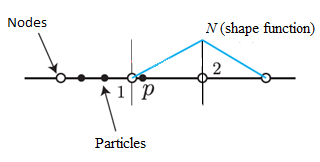
\includegraphics{Hat Function.png}
    	\centering
    	\caption{Hat function on 1-D. Edited from \cite{Nguyen2014}.}
    	\centering
    \end{figure}

\subsubsection{Axial Vibration of a Continuum Bar}
According to \cite{Bardenhagen2002}, the axial vibration of a bar occurs in modes of vibration, which one with different frequency and amplitude of oscillation. Generally, several vibration modes are excited at the same time, however, with specific initial conditions, it is possible to excite a single mode of vibration. The vibration modes are shown in Eq. (16).
\begin{equation}
\phi_n(x)=sin\beta_nx    
\end{equation}

Where $\beta _n$ are the eigenvalues defined according to Eq. (17), where n varies from 1 to infinity and L corresponds to the length of the bar measured in mesh elements.
\begin{equation}
\beta_n = \frac{2n-1}{2}\frac{\pi}{L}    
\end{equation}

The oscillation frequencies, in turn, are defined based on the eigenvalues $\beta_n$ according to Eq. (18).
\begin{equation}
    \omega_n = \beta_nc
\end{equation}

Where c represents the speed of sound in the medium, which can be calculated through the square root of the ratio between the modulus of elasticity of the medium and its density.

Using initial conditions multiples of the systems natural frequency of vibration, it is possible to separately excite the chosen mode of vibration chosen as performed in \cite{Bardenhagen2002} where the conditions used determined that, in the initial instant, the displacement is null in the whole bar and the velocity is defined by Eq. (19), considering a one-dimensional system.

\begin{equation}
    \boldsymbol{v}(x,0)=\boldsymbol{v}_0sin\beta_nx
\end{equation}

Where $\boldsymbol{v_0}$ is the amplitude of the initial velocity.
The problem has an analytical solution for the velocity in the entire domain of the bar, which can be used to develop an expression for the center of mass velocity depending on time Eq. (20).
\begin{equation}
    \boldsymbol{v}_{cm}=\frac{\boldsymbol{v}_0}{\beta_nL}cos(\omega_nt)
\end{equation}

The problem proposed by \cite{Bardenhagen2002} was then reproduced, where a one-dimensional bar fixed at x = 0 and free at x = L vibrates under the aforementioned initial conditions and simulations were performed for three vibration modes (n = 1, 5 and 10). The MPM simulation results for the velocity at the center of mass were then compared to the analytical results from Eq. (20), as performed in \cite{Bardenhagen2002}, using the same input data in the simulation, namely: length of the one-dimensional bar equals to 25, with length of mesh elements $(\Delta x)$ equals to 1, quantity of particles equals to 50, being two per element, modulus of elasticity (E) equals to 100, density $(\rho)$ equals to 1, initial velocity amplitude $(v_0)$ equals to 0.1 and a time increment defined by Eq. (21). The values can be used for any system of measurement.
\begin{equation}
    \Delta t = 0.1\left (\frac{\Delta x}{c}  \right )
\end{equation}

\section{Results}
Figure 2 shows the center of mass velocities according to the analytical result and the one simulated by MPM. The two curves overlap, showing great correspondence of the simulation, as in the work of \cite{Bardenhagen2002}. However, when evaluating the results for the fifth mode of vibration, it is noticed that there is a loss of accuracy. Figure 3 shows the results for n = 5, where it is possible to observe that the curves, although having considerably similar amplitudes, are out of phase. This phase difference is due to the difference between the analytical and simulation frequencies of approximately 5\% of the analytical value. The same behavior was observed in the work of \cite{Bardenhagen2002}. Changes in the number of particles per element did not result in better convergence (with tests being performed for up to 6 particles per element, triple the initial configuration), however, adjustments in the spatial discretization were able to diminish the difference between the frequencies and approximate the results, so that the difference was reduced to approximately 1\% by decreasing the length of the element used in the initial configurations by half. Following the same principle, the results for the tenth mode of vibration, shown in Figure 4, also showed curves with similar amplitudes, but with an even greater phase offset between them. The difference between the analytical and MPM frequencies reached something around 20\%, being this result again consistent with what was found in \cite{Bardenhagen2002}. Again, new simulations varying the number of particles (increasing up to 3 times the initial amount) and the temporal discretization did not result in significant differences, however, adjusting the spatial discretization to half the initial value of the mesh element length made it possible to reduce the difference between frequencies to 5\%.

\begin{figure}
    	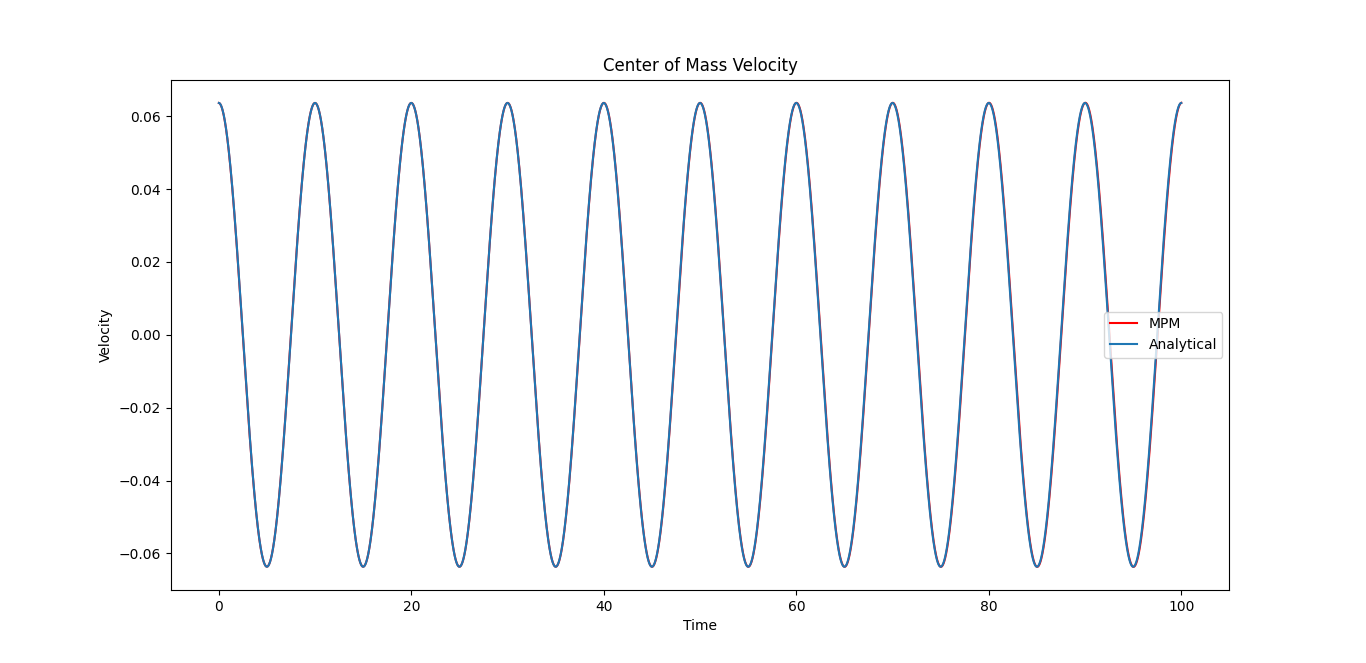
\includegraphics[width=\linewidth]{ModoVibracional1.png}
    	\caption{Mode of vibration 1 – Velocity of the center of mass.}
    	\centering
    \end{figure}

\begin{figure}
    	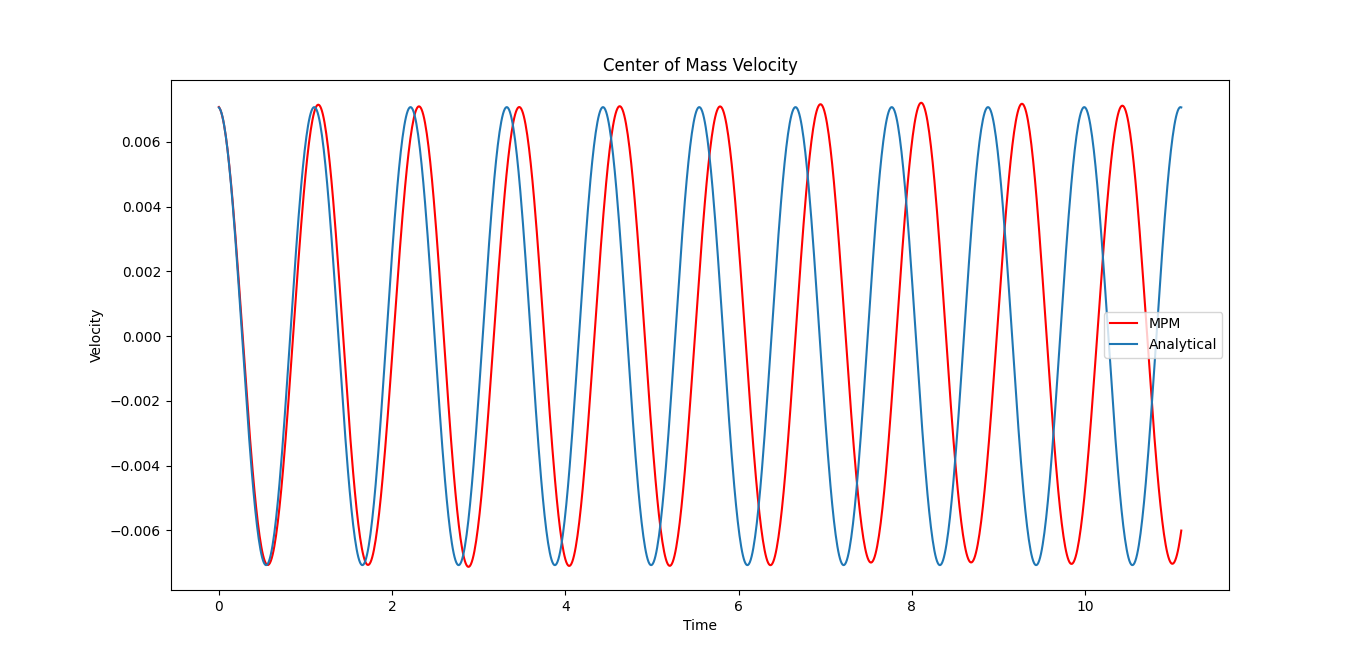
\includegraphics[width=\linewidth]{ModoVibracional5.png}
    	\caption{Mode of vibration 5 – Velocity of the center of mass.}
    	\centering
    \end{figure}

\begin{figure}
    	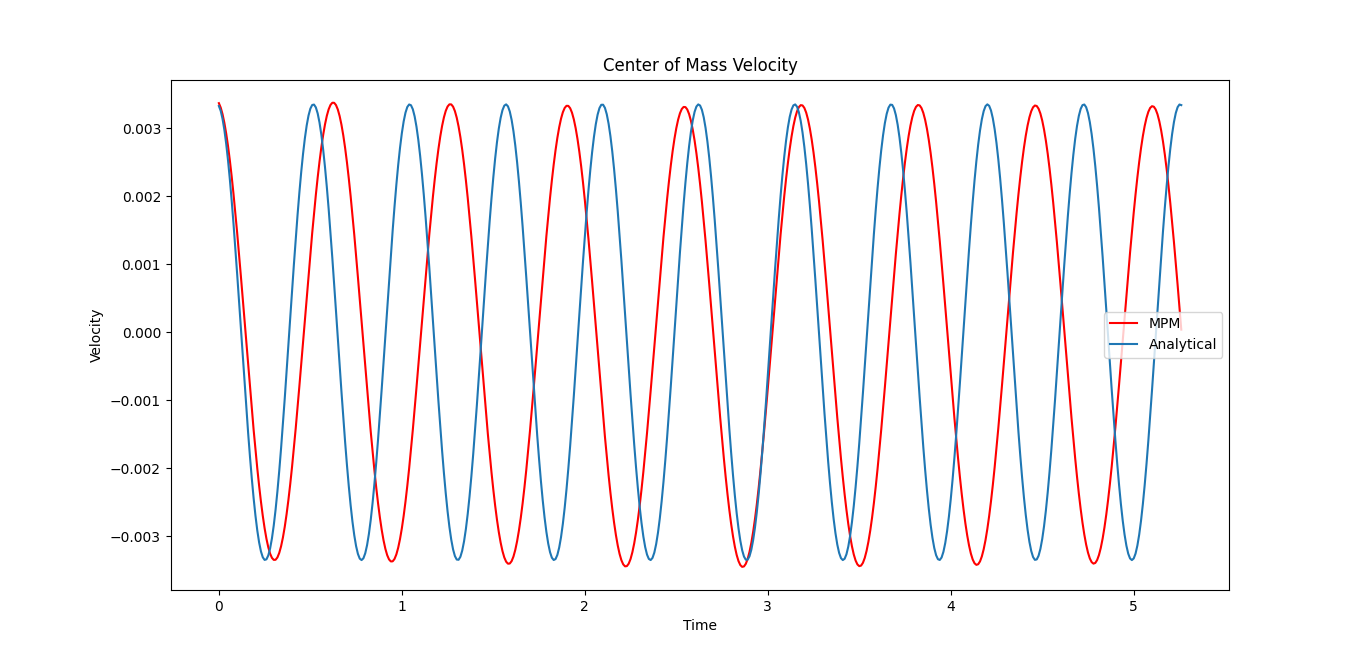
\includegraphics[width=\linewidth]{ModoVibracional10.png}
    	\caption{Mode of vibration 10 – Velocity of the center of mass.}
    	\centering
    \end{figure}

\section{Conclusions}
In this paper carried out an application, for didactic purposes, of the MPM method through the USF algorithm to a one-dimensional system composed of a continuum bar in free axial vibration, as proposed by \cite{Bardenhagen2002}. The results obtained were similar to those found in the literature, with the simulated center of mass velocity being equal to the analytical one in the first mode of vibration and with the phase differences of the remaining modes also corresponding to those reported on \cite{Bardenhagen2002}, indicating that the method was correctly used. For the fifth and tenth modes of vibration, alternative simulations were performed varying the number of particles used, temporal discretization and spatial discretization, the latter being able to reduce the difference between the simulated and analytical frequencies (from 5\% to 1\% in the fifth vibrational pattern; and from 20\% to 5\% in the tenth vibrational mode). From this it is possible to conclude that, despite the results in phase dislocation for n = [5, 10], there is no inadequacy of the numerical method to represent higher order vibration modes, with only the inadequacy of the simulation parameters used, being possible to obtain closer results by adjusting these parameters according to the characteristics of the problem.
%% If you have bibdatabase file and want bibtex to generate the
%% bibitems, please use
%%
 \bibliographystyle{elsarticle-num} 
 \bibliography{cas-refs}

%% else use the following coding to input the bibitems directly in the
%% TeX file.

% \begin{thebibliography}{00}

% %% \bibitem{label}
% %% Text of bibliographic item

% \bibitem{}

% \end{thebibliography}
\end{document}
\endinput
%%
%% End of file `elsarticle-template-num.tex'.
